% Options for packages loaded elsewhere
\PassOptionsToPackage{unicode}{hyperref}
\PassOptionsToPackage{hyphens}{url}
%
\documentclass[
]{book}
\usepackage{amsmath,amssymb}
\usepackage{lmodern}
\usepackage{iftex}
\ifPDFTeX
  \usepackage[T1]{fontenc}
  \usepackage[utf8]{inputenc}
  \usepackage{textcomp} % provide euro and other symbols
\else % if luatex or xetex
  \usepackage{unicode-math}
  \defaultfontfeatures{Scale=MatchLowercase}
  \defaultfontfeatures[\rmfamily]{Ligatures=TeX,Scale=1}
\fi
% Use upquote if available, for straight quotes in verbatim environments
\IfFileExists{upquote.sty}{\usepackage{upquote}}{}
\IfFileExists{microtype.sty}{% use microtype if available
  \usepackage[]{microtype}
  \UseMicrotypeSet[protrusion]{basicmath} % disable protrusion for tt fonts
}{}
\makeatletter
\@ifundefined{KOMAClassName}{% if non-KOMA class
  \IfFileExists{parskip.sty}{%
    \usepackage{parskip}
  }{% else
    \setlength{\parindent}{0pt}
    \setlength{\parskip}{6pt plus 2pt minus 1pt}}
}{% if KOMA class
  \KOMAoptions{parskip=half}}
\makeatother
\usepackage{xcolor}
\IfFileExists{xurl.sty}{\usepackage{xurl}}{} % add URL line breaks if available
\IfFileExists{bookmark.sty}{\usepackage{bookmark}}{\usepackage{hyperref}}
\hypersetup{
  pdftitle={Wenzhou-Kean University Data Analysis Bootcamp Series},
  pdfauthor={Chungil Chae(Chad)},
  hidelinks,
  pdfcreator={LaTeX via pandoc}}
\urlstyle{same} % disable monospaced font for URLs
\usepackage{longtable,booktabs,array}
\usepackage{calc} % for calculating minipage widths
% Correct order of tables after \paragraph or \subparagraph
\usepackage{etoolbox}
\makeatletter
\patchcmd\longtable{\par}{\if@noskipsec\mbox{}\fi\par}{}{}
\makeatother
% Allow footnotes in longtable head/foot
\IfFileExists{footnotehyper.sty}{\usepackage{footnotehyper}}{\usepackage{footnote}}
\makesavenoteenv{longtable}
\usepackage{graphicx}
\makeatletter
\def\maxwidth{\ifdim\Gin@nat@width>\linewidth\linewidth\else\Gin@nat@width\fi}
\def\maxheight{\ifdim\Gin@nat@height>\textheight\textheight\else\Gin@nat@height\fi}
\makeatother
% Scale images if necessary, so that they will not overflow the page
% margins by default, and it is still possible to overwrite the defaults
% using explicit options in \includegraphics[width, height, ...]{}
\setkeys{Gin}{width=\maxwidth,height=\maxheight,keepaspectratio}
% Set default figure placement to htbp
\makeatletter
\def\fps@figure{htbp}
\makeatother
\setlength{\emergencystretch}{3em} % prevent overfull lines
\providecommand{\tightlist}{%
  \setlength{\itemsep}{0pt}\setlength{\parskip}{0pt}}
\setcounter{secnumdepth}{5}
\usepackage{booktabs}
\ifLuaTeX
  \usepackage{selnolig}  % disable illegal ligatures
\fi
\usepackage[]{natbib}
\bibliographystyle{plainnat}

\title{Wenzhou-Kean University Data Analysis Bootcamp Series}
\author{Chungil Chae(Chad)}
\date{2021-11-26}

\begin{document}
\maketitle

{
\setcounter{tocdepth}{1}
\tableofcontents
}
\hypertarget{about-bootcamp-series}{%
\chapter{About Bootcamp Series}\label{about-bootcamp-series}}

\emph{Organizer: WKU Library}

\begin{itemize}
\tightlist
\item
  Session1: Bootcamp R: Basic Social Network Analysis and Dynamic Reporting with R

  \begin{itemize}
  \tightlist
  \item
    CBPM A102
  \item
    Nov 27 (SAT)
  \item
    10:30 AM
  \end{itemize}
\item
  Session2: Bootcamp Stata: Database Introduction Data Analysis

  \begin{itemize}
  \tightlist
  \item
    Location (TBA)
  \item
    Date (TBA)
  \item
    Time (TBA)
  \end{itemize}
\end{itemize}

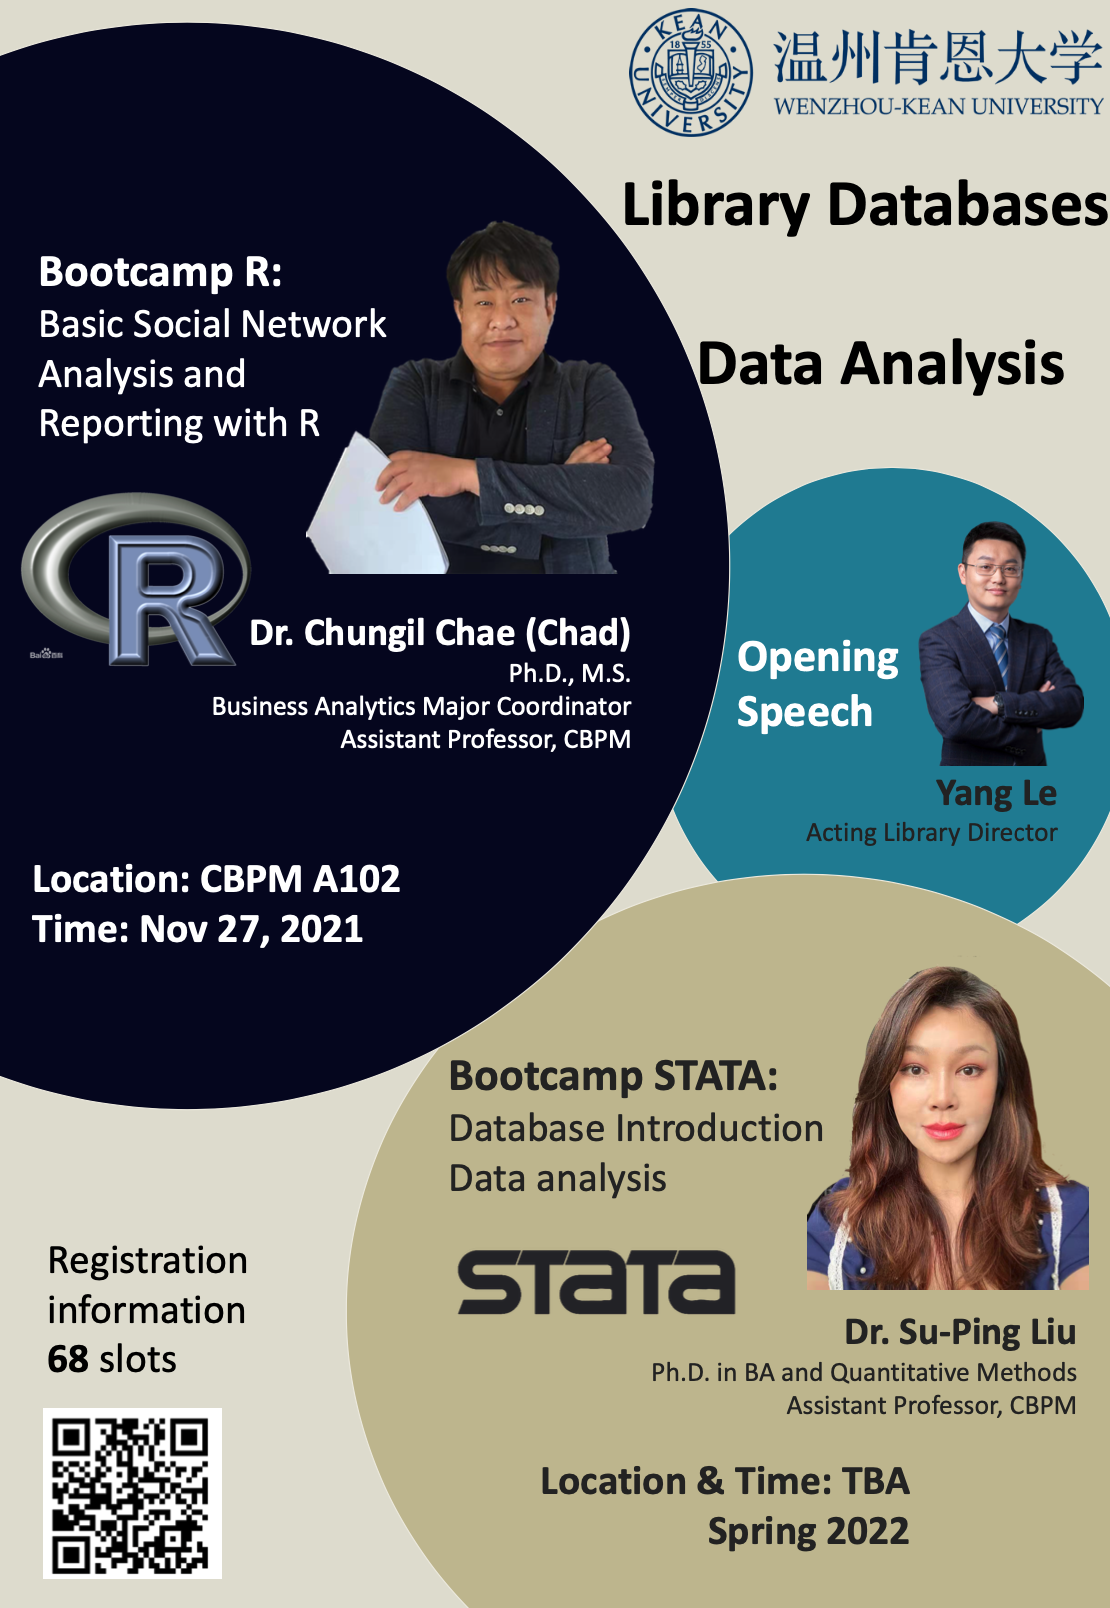
\includegraphics[width=6.25in,height=\textheight]{images/0.png}

\hypertarget{objective-and-introduction}{%
\section{Objective and Introduction}\label{objective-and-introduction}}

The Bootcamp is addressed to undergraduate students at Wenzhou-Kean University. It represents a unique opportunity to attend lectures on library database exploration and data analysis instructed by expert faculty and receive feedback both on developed (senior theses) and developing projects (early-stage ideas).

\hypertarget{bootcamp-r-basic-social-network-analysis-and-dynamic-reporting-with-r}{%
\chapter{Bootcamp R: Basic Social Network Analysis and Dynamic Reporting with R}\label{bootcamp-r-basic-social-network-analysis-and-dynamic-reporting-with-r}}

This bootcamp aims to introduce dynamic documentation in R and basics of social network analysis in R

\hypertarget{program}{%
\section{Program}\label{program}}

\begin{itemize}
\tightlist
\item
  Session 1: Bootcamp R: Basic Social Network Analysis and Reporting with R
\item
  Saturday, November 27, Fall 2021

  \begin{itemize}
  \tightlist
  \item
    10:30-11:00 (CBPM A102):

    \begin{itemize}
    \tightlist
    \item
      Opening Speech (Le Yang, Acting Library Director)
    \end{itemize}
  \item
    11:00-12:30 (CBPM A102):

    \begin{itemize}
    \tightlist
    \item
      Basics of R and Generating Report with R markdown
    \end{itemize}
  \item
    12:30-13:30: Lunch
  \item
    13:30-16:00 (CBPM A102):

    \begin{itemize}
    \tightlist
    \item
      Basics of Social Network Analysis
    \end{itemize}
  \item
    16:00-16:30 (GEH A301):

    \begin{itemize}
    \tightlist
    \item
      Digital Scholarship Center Tour
    \end{itemize}
  \end{itemize}
\end{itemize}

\hypertarget{requirement}{%
\section{Requirement}\label{requirement}}

\begin{itemize}
\tightlist
\item
  Personal Labtop
\end{itemize}

\hypertarget{assistants}{%
\section{Assistants}\label{assistants}}

\hypertarget{yuliana-yuejiu-zhang}{%
\subsection{Yuliana (Yuejiu Zhang)}\label{yuliana-yuejiu-zhang}}


\includegraphics{image/ta_yul.png}

\begin{quote}
Yuejiu Zhang is a junior accounting student of Wenzhou-Kean University. She also experienced the business competition on the campus and won the Third Prize of Wenzhou-Kean University First ``social Dag Cup'' management rights competition
\end{quote}

\begin{center}\rule{0.5\linewidth}{0.5pt}\end{center}

\hypertarget{tony-jiongcheng-lu}{%
\subsection{Tony (Jiongcheng Lu)}\label{tony-jiongcheng-lu}}

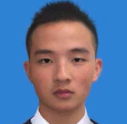
\includegraphics{image/ta_to.png}

\begin{quote}
Tony (Jiongcheng Lu) is a junior student major in Finance who takes a teaching assistant responsibility for MGS3001/Section1 Python Programming for Business in 2021, summer semester. Tony's study concentrates on Data Analytics and Finance. Tony aims to apply data analytics techniques to in-depth analysis for a financial institution.
\end{quote}

\begin{center}\rule{0.5\linewidth}{0.5pt}\end{center}

\hypertarget{jason-shiyu-jiang}{%
\subsection{Jason (Shiyu Jiang)}\label{jason-shiyu-jiang}}


\includegraphics{image/ta_ja.png}

\begin{quote}
Shiyu Jiang (Jason) is a junior in computer science and technology. He takes a teaching assistant responsibility for MGS 3001 Python Programming for Business in 2021 Spring semester. Jason focuses mainly on data science and big data development. He has lead or took part in several research projects launched by professors in WKU and Chinese Academy of Science.
\end{quote}

\hypertarget{materials}{%
\section{Materials}\label{materials}}

\begin{itemize}
\tightlist
\item
  \href{https://github.com/chadchae/ws_ba_bootcamp_2021/blob/master/products/snabootcamp.R}{R Source Code}
\item
  \href{https://github.com/chadchae/ws_ba_bootcamp_2021/blob/master/products/snabootcamp.pdf}{Presentation}
\end{itemize}

\hypertarget{bootcamp-stata-database-introduction-data-analysis}{%
\chapter{Bootcamp Stata: Database Introduction Data Analysis}\label{bootcamp-stata-database-introduction-data-analysis}}

TBA

\end{document}
